%!TEX root = ../thesis.tex
%*******************************************************************************
%*********************************** First Chapter *****************************
%*******************************************************************************


\chapter{Introduction and literature review}


\ifpdf
    \graphicspath{{Chapter1/Figs/Raster/}{Chapter1/Figs/PDF/}{Chapter1/Figs/}}
\else
    \graphicspath{{Chapter1/Figs/Vector/}{Chapter1/Figs/}}
\fi

%*******************************************************************************

\section[Research outline and background]{Research outline and background} % 4300 words in intro as of sept 22
\label{section1.1}

\subsection[Research outline and goals]{Research outline and goals}
\label{subsection1.1.1}

This research concerns chemical and morphological differences between natural azurite and synthetic verditer pigments. Early modern English vernacular wall paintings are the central aspect of material culture that will be studied. However, disruption from COVID-19 pandemic has affected sample availability, and additional work on easel painting cross sections and natural azurite reference samples has been the initial focus. The research to date and the future directions of work are outlined.

Initial work has established sample preparation and analysis parameters for Raman spectroscopy, SEM-EDS, and AFM-IR. Thirteen reference samples of powdered azurite, malachite, and verditers have been provided by the Hamilton Kerr Institute and Dr. Andrea Kirkham. Analysis of these samples comprises the bulk of this report and establishes basic expectations of sample morphology and constituent element variation. SEM and AFM imaging provide information about morphology, and SEM, EDS, and Raman spectroscopy identify minerals present.

Additional samples are needed to build a comprehensive library of information about natural azurite and synthetic verditer. To that end, natural azurite samples have been procured from the Sedgwick Museum of Earth Sciences and will by fully characterised. Additional samples of natural azurite and synthetic verditer will be studied in easel painting cross sections from the HKI.

A collaboration with Katherine Waldron at the Hamilton Kerr Institute began in July 2021. Twelve cross sections from \textit{The Battle of Spurs} (c. 1513, Hampton Court Palace) containing azurite were analysed using SEM-EDS. This provided information about associated minerals found in azurite used in England during the 16th century, albeit in the context of elite easel painting rather than vernacular wall painting. Pigment size and morphology were also studied across different areas of the painting aiming to determine the consistency of historical pigment grinding and purification procedures. This painting has not been scientifically analysed to date.

Future work will continue to focus on geologic samples and cross sections containing azurite and verditer pigments. Wall painting samples will be studied by the same methods. If there is an opportunity for microdestructive testing, ToF-SIMS analysis would be useful in the study of heavy metals, but this is not an option for cross sections. The viability of historically relevant synthetic syntheses for verditer will be determined.

\subsection[History of early modern English wall paintings]{History of early modern English vernacular wall paintings}
\label{subsection1.1.2}

From the mid 1500s to early 1600s, elaborate wall paintings were popular around England and Wales across all classes with disposable income.~\autocite{Baird_thesis,Davies_book,Kirkham_thesis} Two recent comprehensive studies have been carried out, by Kirkham in Suffolk/Norfolk and by Baird/Davies in the Welsh Marches. Although this trend was short-lived, it is significant because it appeared during a period of other significant changes in English society. Increased social mobility and increasing numbers of lesser gentry resulted in instability in defining class and status.~\autocite{Baird_thesis,Hamling_book} Wall paintings are understood to be a means of communicating status during this period.~\autocite{Baird_thesis,Davies_book,Kirkham_thesis}

During this period, historians observe a movement away from the Medieval open hall to houses with smaller rooms with specific purposes and greater privacy.~\autocite{Baird_thesis,Davies_book,Hamling_book} The Reformation led to destruction of religious images in churches and restricted the subjects considered ideologically acceptable in secular buildings.~\autocite{Kirkham_thesis,Hamling_book,Giles} Finally, trade with the continent and the printing press allowed wide dissemination of images and trends. These social changes are important for contextualizing wall paintings. Wall paintings offer a rare view into the choices and fashions of the middling class during a period of upheaval.~\autocite{Kirkham_thesis,Baird_thesis} However, many paintings do not survive due to destruction or overpainting, and have been neglected in spite of the information they contain about how social status was communicated and gained, and how people conceived of the home.~\autocite{Benton1,Benton2,Kirkham_thesis}

%Wall paintings were characterized by a range of quality and aesthetic appeal. Floral/foliate motifs, antiquework designs originating from Italy, and arabesques were widely used.~\autocite{Kirkham_thesis,Baird_thesis,Thornton_book} Fewer figurative and religious subjects are observed, particularly in Suffolk. Many schemes imitated textiles and wood panelling, both unaffordable for middling folk. Many paintings also incorporated texts into imitation textiles or with decorative borders.~\autocite{Baird_thesis,Kirkham_thesis} Texts were often placed over fireplaces or over doors, and were used to teach morals.~\autocite{Hamling_book} 

The cost of wall painting schemes depended on the cost of materials such as pigments as well as labour.~\autocite{Baird_thesis,Davies_book,Kirkham_thesis} Pigments were selected based on cost and aesthetic effect.~\autocite{Kirkham_thesis} Kirkham suggests that blue verditer may have been selected because it was a newly available, fashionable pigment. It was often used in urban schemes in Suffolk rather than in rural areas, and has not been found in the Welsh Marches.~\autocite{Kirkham_thesis,Baird_thesis} This may be due to availability related to commerce links with London and the continent or local trends. Blue rooms were fashionable at the time, influenced by French court styles, and the presence of a blue room in an early modern house marked elite status or aspirations.~\autocite{Kirkham_thesis}

\subsection[Historical use of blue pigments in wall paintings]{Historical use of blue pigments in wall paintings}
\label{subsection1.1.3}

The use of blue pigments during this period is of interest due to their limited availability and high cost. There were four blue pigments available to vernacular painters - indigo/woad, blue verditer, smalt, and azurite. Azurite was not widely observed at the vernacular level, and ultramarine was not used at any level for decorate painting due to rarity and cost.~\autocite{Kirkham_thesis} While only indigo/woad were observed in the Welsh Marches, blue verditer and (rarely) azurite were observed in the East of England.~\autocite{Baird_thesis,Davies_book,Kirkham_thesis} Smalt, a crushed glass, was difficult to work with and not used extensively.~\autocite{Kirkham_thesis}

Azurite is a naturally occurring basic copper carbonate with the chemical formula Cu\textsubscript{3}(CO\textsubscript{3})\textsubscript{2}(OH)\textsubscript{2}.~\autocite{Aru,Smieska} It forms around copper deposits and was mined during this period in eastern Europe.~\autocite{Aru} It has been used since antiquity, observed in Egyptian art and Medieval European illuminated manuscripts.~\autocite{Smieska} Seldes et al. identified azurite in 18th century South American paintings, where the pigment was called ``blue powder" or ``blue ashes."~\autocite{Seldes} Clarke et al. identified azurite in 13th century Japanese scroll paintings.~\autocite{Clarke} Many mineral impurities are observed in natural azurite formations, and these as well as particle size variation affect the colour and visual effect of the pigment.~\autocite{Smieska,Price,Cardell}

Blue verditer is the synthetic analogue of azurite and has been identified in wall paintings dating to the early 1600s (1610-1620 as earliest approximate date of use). In Kirkham's study of wall paintings in Suffolk country, blue verditer was found in several elaborate decorative schemes and in the inventories of painters, merchants, and grocers. The cost of blue verditer depended on quality; slightly less expensive than indigo and significantly less than the lowest grade of azurite.~\autocite{Kirkham_thesis} 

Blue verditer was a by-product of gold refining, but was challenging to produce to high quality standards. The sources of historical verditer are not known, though Kirkham suggests the Netherlands as a possible source.~\autocite{Kirkham_thesis,Kirby} Identification of artificial blue and green pigments by scientific methods has not been widely undertaken. Naumova et al.'s studies of Russian frescoes is one example but does not employ recent advances in chemical analysis.~\autocite{Naumova1994,Naumova1990}

Recipes purporting to produce blue and green copper-based pigments date to Ancient Greece and the medieval period.~\autocite{mappae_clavicula, Orna_literature, Orna_silver, Barnett} Orna et al. evaluated medieval recipes claiming to produce blue pigment from the treatment of silver and copper metals. Treatment of copper containing alloys with acetic acid formed verdigris and copper acetate, but copper carbonates were not observed.~\autocite{Orna_literature,Orna_silver}

MacTaggart et al. studied recipes for producing blue and green verditers, synthetic analogues of azurite and malachite. Blue verditer is also called ``blue bice" and ``blue ashes." They discussed characteristics of historical verditers, ``tiny, rounded, fibrous aggregates, even in size, highly birefracting, and blue by transmitted light." There are credible historical references to verditers dating to the early 1500s, and they claim that blue verditer was a speciality of English producers at this time. However, the authors note that blue verditer was also used as a general term for any blue pigments regardless of composition or production. 

To determine a successful method for producing verditers that meet previously identified physical markers, they tested the procedure for refining gold for which blue verditer was a by-product. Ultimately, they struggled to consistently produce blue verditer, as did early modern refiners, and they proposed that the success of synthesis was dependent on the weather; blue particles were only produced at temperatures below 12 \textdegree C.~\autocite{MacTaggart}
%- color dependence on grain size - smieska, painting manuals, that other ref about separating the sizes, cardell, price

\subsection[Open research questions about wall paintings]{Open research questions about wall paintings and early modern material culture}
\label{subsection1.1.4}

This research is concerned with the open questions relating to the materiality of wall paintings. Scientific research into the materials used by craftsmen has been limited.~\autocite{Baird_thesis, Davies_book} Availability of various blue (and, to a lesser extent, green) pigments during this period has been debated, and the language used to describe blue pigments is inconsistent and scientifically inaccurate.~\autocite{Harley} 

The use of synthetic copper carbonate blue pigments (blue verditer) has been noted in Suffolk.~\autocite{Baird_thesis, Kirkham_thesis} This discovery must be corroborated and a larger body of samples should be analysed to determine the extent of use. This matters in the interpretation of the purpose, cost, value, and disposability of wall paintings.~\autocite{Baird_thesis,Davies_book} The availability of synthetically produced pigments to the middling class could indicate new industrial methods of production and close ties between scientists, artists, and craftsmen. 

This work also has important implications for preservation and restoration of these works, often in poor condition or at risk of being lost. Many vernacular wall paintings from this period have been demolished despite their importance to our understanding of daily life during the period.~\autocite{Davies_book,Hamling_book,Benton1,Benton2} Azurite and verditer pigments are unstable and can be altered by excessive humidity and alkalinity, as well as light exposure, and this research could inform future preservation and restoration choices.~\autocite{Saunders,Cardell,Lluveras,Mattei,Dei}


\subsection[Previous scientific work on copper carbonate pigments]{Previous scientific work on copper carbonate pigments}
\label{subsection1.1.5}

Previous work characterised azurite, malachite, and their degradation products using confocal Raman spectroscopy and infrared spectroscopy. Production and use of synthetic blue and green pigments in England and continental Europe has been studied minimally. Synthetic recipes from the medieval period have been evaluated for their success in producing pigments.

Frost et al. studied malachite and azurite using confocal/polarised Raman spectroscopy, assigning peaks and determining orientation dependence in spectra.~\autocite{Frost} Bicchieri et al. studied lapis lazuli and azurite pigments on parchment using micro-Raman and laser induced breakdown spectroscopies.~\autocite{Bicchieri} 

Saunders et al. studied the changes azurite undergoes upon exposure to high humidity, noting that azurite has been observed to degrade to malachite or green copper chlorides. They found that azurite was largely unaffected by light under all humidity conditions, with one sample forming copper chlorides when exposed to NaCl and one inexplicably darkening.~\autocite{Saunders} Cardell et al. determined that azurite was altered by natural (outdoor) and artificial ultraviolet light exposure, dependent upon pigment grain size.~\autocite{Cardell} Lluveras et al. mapped green degradation products using synchrotron radiation, determining that copper oxalates and copper hydroxychlorides formed in different areas of the azurite surface depending on proximity to calcium and chlorine ions.~\autocite{Lluveras} The chemical heterogeneity observed here supports the use of surface analytic techniques.

Mattei et al. studied heat and alkaline-induced azurite degradation. They found that azurite is unstable, degrading easily to form malachite, to Cu\textsubscript{2}Cl(OH)\textsubscript{3} (atacamite, paratacamite or clinoatacamite), or less often to CuS or CuO (tenorite). Tenorite was found following heating of azurite particles, and degradation depended on pigment grain size. Tenorite was also found following exposure to alkaline terra cotta. They did not discuss alterations to crystal structure or measure the depth of penetration into the sample.~\autocite{Mattei} 

Naumova et al. studied the green pigments used in medieval Russian frescoes dating to the 1500s, and identified several synthetic pigments for which recipes from the period are not known. They note that artificial pigments were circular in grain shape and showed a characteristic black cross when viewed under a polarised microscope through crossed nicol prisms. However, these identifiers were noted to be problematic and inaccurate at times. Naumova et al. attempted to recreate historical recipes for blue and green pigments, and were unable to synthetically produce azurite. This is one of few sources that does discuss the use of synthetic pigments, and concludes that further research is necessary in this area.~\autocite{Naumova1994,Naumova1990}

Aru et al. characterised the mineral impurities present in azurite samples from mines active during the medieval period using Raman spectroscopy. Many associate minerals were discovered, including malachite, hematite, goethite, cuprite, and titanium dioxides. Quartz, calcite, cerussite, orthoclase, beudantite and jarosite were less common. Tenorite, identified by Aru et al. as a degradation product, was not identified as an impurity in these samples. Unfortunately, though the samples were collected from mines that were active during the medieval period, they dated at the earliest to the eighteenth century, and the small sample size precludes the use of impurities to conclusively trace provenance.~\autocite{Aru} However, this research suggests that the presence of trace minerals is indicative of environmental conditions when azurite crystals form, and that these minerals should be studied using a larger sample set to identify patterns in their occurrence. This supports the use of techniques that detect surface heterogeneity and suggests that mineral inclusions will differ in natural versus artificial samples.

Pigment interactions with organic binders and plaster materials have been studied. Dei et al. studied the production of paratacamite, a green copper chloride, as a degradation product of azurite pigment used in Renaissance Italian frescoes.~\autocite{Dei} Gunn et al. studied darkening of azurite and malachite pigments in oil-based binding media due \textit{via} binding of copper ions by fatty acids.~\autocite{Gunn} Linke et al. studied an unusual violet coloured degradation product of a copper carbonate mixed with casein and applied to plaster.~\autocite{Linke}


%Odlyha - Dosimetry of paintings: Determination of the degree of chemical change in museum exposed test paintings (smalt tempera) by thermal analysis

%Scott - A Review of Copper Chlorides and Related Salts in Bronze Corrosion and as Painting Pigments


\section[Methodology and theoretical background]{Methodology and theoretical background}
\label{section1.2}

\subsection[Confocal Raman spectroscopy]{Confocal Raman spectroscopy}
\label{subsection1.2.1}

Raman spectroscopy uses the interactions between photons from an incident laser beam and molecules or particles in the sample to identify functional groups and other molecular structures. Incident photons at a specific frequency with energy $E_{in} = h\nu$ are directed at the surface of the sample, where they scatter back and are detected. Most photons are scattered back at the same energy, undergoing elastic collisions; this is known as Rayleigh scattering. Some return at higher energies (Anti-Stokes scattering) or lower energies (Stokes scattering). In the case of Stokes scattering:

\begin{equation} \label{eq:raman_1}
E_{out} = E_{in} - \Delta E
\end{equation}

with $E_{out}$ as the energy of the photon that returns from the sample surface. Stokes scattering is more common than Anti-Stokes scattering because the vast majority of sample molecules are in their ground vibrational state at room temperature. This means that they do not have excess vibrational energy to transfer to the incident photon. $\Delta E$ is the change in energy between the ground ($E_{g}$) and excited ($E_{ex}$) vibrational states:

\begin{equation} \label{eq:raman_2}
\Delta E = E_{ex} - E_{g}
\end{equation}

This change in energy $\Delta E$ is known as the Raman shift. Different bonds have different Raman shifts, and the Raman shift is also affected by the chemical environment of the bond. The technique can identify not only different molecules and compounds in a sample, as they each produce a distinct Raman spectrum, but also chemical and structural variation.~\autocite{2018RS,horiba,matousek_tissue} Changing chemical environments induce shifts in peak centres as well as broadening. Relative peak intensities can indicate degrees of disorder or the loss of specific types of bonds or functional groups.~\autocite{tomasini_raman} The selection rules for a bond to be Raman-active require perturbation of the polarisability (or transient dipole) of the molecule.~\autocite{2018RS,inphotonics}
%, while the selection rules for infrared activity require perturbation of the dipole moment

Raman spectroscopy is widely used in conservation science. Analysis can be nondestructive, and informs about both inorganic and organic materials.~\autocite{conti_2016} Raman spectroscopy has been used to study pigments and binders, identify chemical species, and monitor changes due to ageing and environmental exposure as well as pigment-binder interactions.~\autocite{conti_2016, matousek_tissue, tomasini_raman, pallipurath2014, pallipurath2013, lazzari, vandenabeele} 

Raman spectroscopy has limitations, particularly when studying samples which fluoresce at the selected Raman excitation wavelength. Broad, intense fluorescence bands mask the weaker scattering from the sample.~\autocite{Wei} It is possible to shift the fluorescence bands to a frequency outside of the region of interest by using a different excitation wavelength, often by moving to a near-infrared rather than a visible light excitation.~\autocite{Kaszowska,Mancini} However, this also affects the risk of damage and the Raman efficiency observed. Many organic binders and some pigments fluoresce, so this remains a challenge. 


\subsection[Scanning electron microscopy and energy dispersive spectrometry]{Scanning electron microscopy and energy dispersive spectrometry}
\label{subsection1.2.2}

Scanning electron microscopy (SEM) has been used to study art and heritage objects. Painting cross sections, ceramic glaze structures, and archaeological artefacts are often investigated by SEM, as are relevant chemical processes such as surface degradation and formation of undesirable breakdown products such as metal soaps.~\autocite{Lazzara, Hermans, Pradell, Schreiner} SEM is coupled to energy dispersive spectroscopy (EDS), providing quantitative detection and spatial resolution of elements.

SEM offers sub-diffraction-limit resolution imaging, meaning that magnifications can be reached that exceed the maximum of an optical microscope. An electron beam accelerated at a set voltage interacts with the sample. These electrons may scatter, reflect, or transmit through the sample. They may also induce emission of secondary electrons or X-rays from the sample. X-rays are emitted at characteristic energies, detected using EDS to give information about elemental composition. Backscattered beam electrons are detected at energies dependent on atomic weight using a backscatter (BS) detector to construct a map of the sample with stronger intensities in areas composed of heavier elements.~\autocite{Lazzara,Pradell,Schreiner} Secondary electrons are detected using a secondary electron (SE) detector to construct a three-dimensional topographic map of the sample. Typical resolutions of BS and SE detectors are on nanometer scale, while typical resolutions of EDS detectors are micron scale.~\autocite{Lazzara}

There are limitations in instrument capabilities and sampling restrictions. Small sample chambers, chamber vacuum pressures, and surface charging issues may limit the ability to carry out nondestructive analysis. SEM-EDS cannot identify crystal structure, which requires X-ray diffraction experiments.~\autocite{Lazzara,Schreiner} EDS is also limited in its ability to detect elements lighter than carbon, and while it is generally quantitative for trace elements, background noise means that elements present at levels below 0.1\% abundance are not detectable.~\autocite{Schreiner,Pradell,Lazzara} Several elements have EDS peaks which appear at similar energies. This hinders identification, particularly when these peaks are assignable to multiple expected sample components.


\subsection[Atomic force microscopy]{Atomic force microscopy}
\label{subsection1.2.3}

Atomic force microscopy (AFM) coupled to infrared spectroscopy is a novel analytic method for studying surfaces below the diffraction limit.~\autocite{dazzi2017,kurouski} It has been used previously to study artworks and heritage objects. Latour et al. studied degradation of collagen in parchments, Morsch et al. have investigated heterogeneity of epoxy surfaces and linseed oil interactions with titanium dioxide pigment, and Ma et al. studied the formation of metal carboxylate salts in oil paint.~\autocite{latour,Morsch,morsch2016,ma} Barberio et al. have shown that AFM is useful in determining the degradation state and patina on stone artefacts using significantly smaller samples than are required for traditional petrographic analysis.~\autocite{Barberio} Most significantly, AFM-IR has only microdestructive sampling requirements and provides a great deal of information about the physical and chemical properties of surfaces.~\autocite{dazzi2017,kurouski}

Conventional infrared spectroscopy has an inherent resolution limit related to the wavelength of incident light; the diffraction limit for an incident beam of $\lambda$ is $\lambda$/2. Typically, this is approximately several hundred nanometers to several microns. AFM, on the other hand, uses a narrow physical probe to investigate properties of the sample instead. This means that the resolution is limited to the size of the probe, and can be as small as sub-20 nm.~\autocite{dazzi2017} In addition to studying the friction, roughness, and topography of the sample surface using physical probe-surface interactions, recent work has coupled the high resolution of AFM to infrared spectroscopy providing information about chemistry of the surface.~\autocite{dazzi2017,kurouski}

When the AFM probe interacts with the surface, the cantilever is deflected and, like a spring, oscillates. A laser that is reflected off the cantilever into a detector registers the oscillation. Images can be collected in tapping mode, where the probe is not constantly in contact with the surface, or in contact mode where the tip moves along the surface maintaining the interaction. Surface friction is measured using the side-to-side deflection of the tip in contact mode.~\autocite{friction_afm} Infrared spectra are collected by measuring the probe displacement due to thermal expansion of the sample, caused by incoming infrared radiation.~\autocite{dazzi2017,kurouski} The infrared collection system is shown in \textit{Figure \ref{fig:afm_diagram}}.

\begin{figure}[H]
\centering
  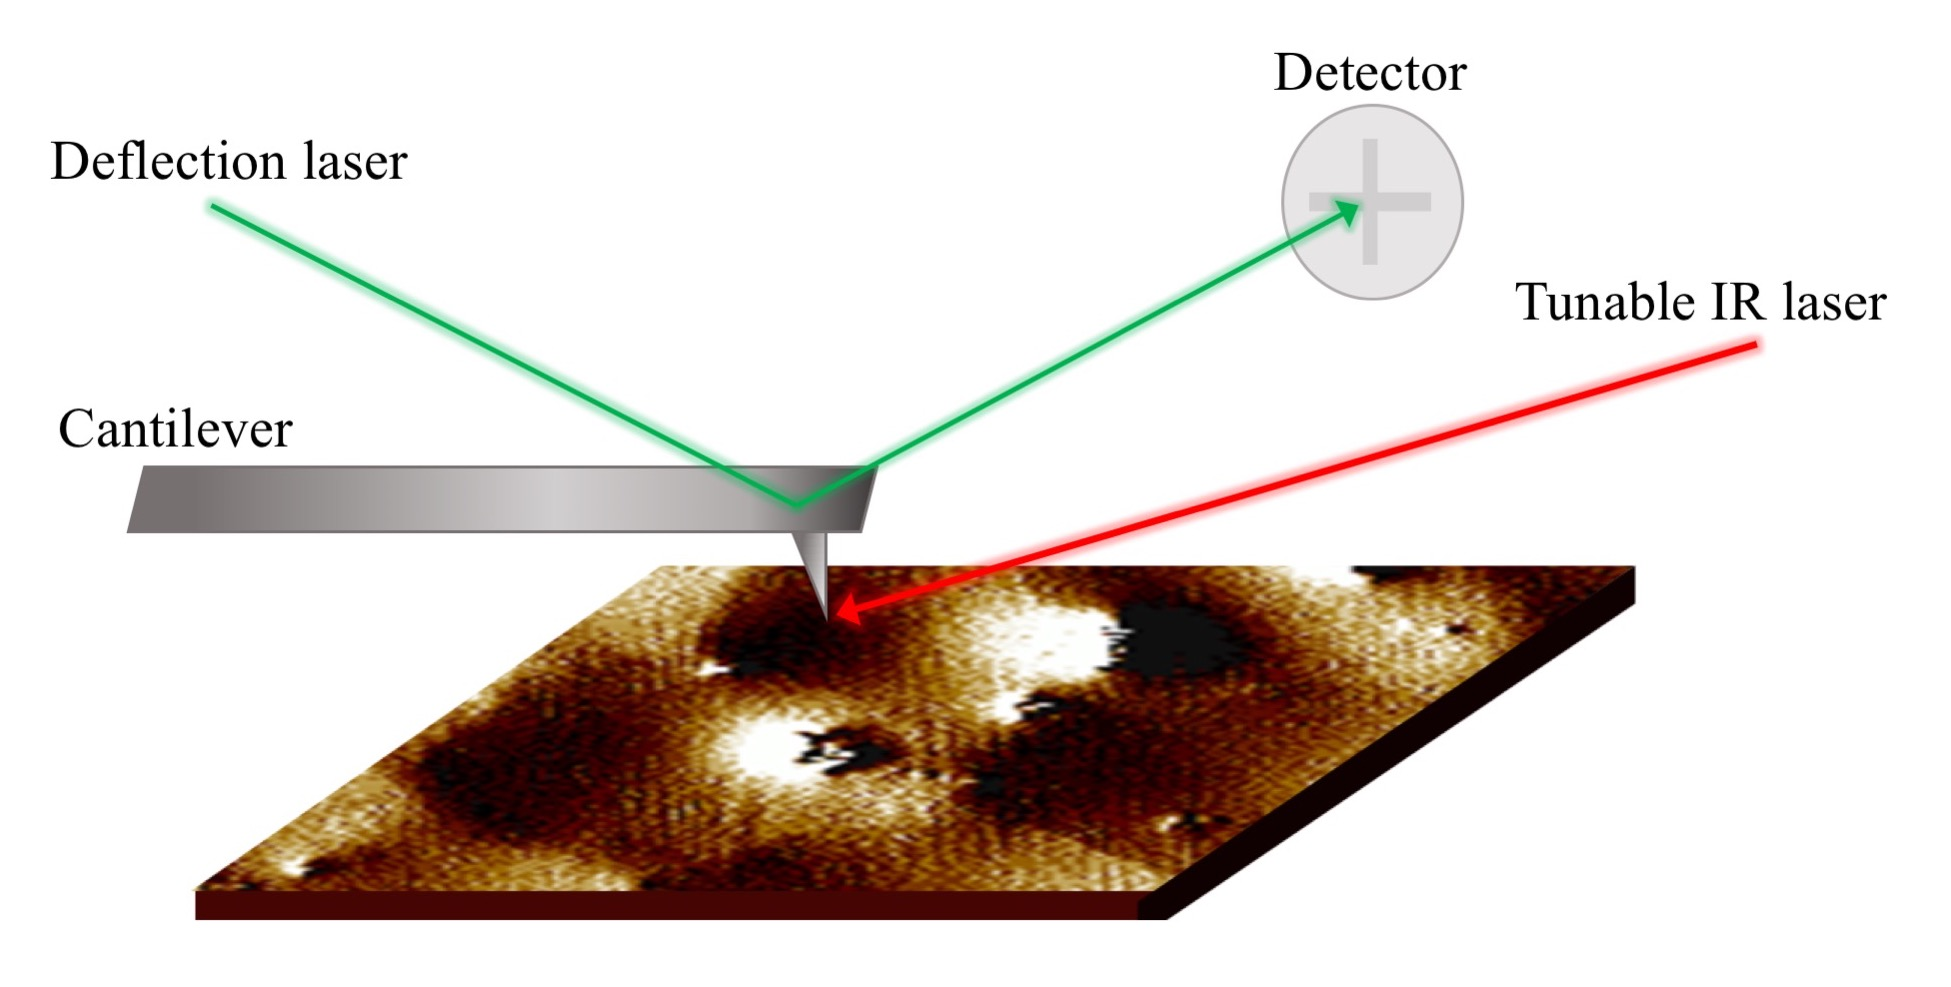
\includegraphics[width=\linewidth]{afm_diagram}
\caption[Diagram of AFM-IR schematic showing a top-down illumination system.]{Diagram of AFM-IR schematic showing a top-down illumination system. The incident infrared beam causes the sample to expand and move the probe-cantilever system. The cantilever deflection is recorded and detected by another laser beam reflected into a photodiode detector.~\autocite{Morsch,dazzi2017} Figure is reproduced from Masters thesis, \textit{Spectroscopic Analysis of Thin Oil Paint Films and Oxidation Processes}, Ellen Purdy (2021).}
\label{fig:afm_diagram}
\end{figure}

AFM-IR spectra are directly comparable to conventional IR spectra because the oscillations of the cantilever are proportional to the absorption coefficient of the sample. This means that peak locations and band shapes will not be affected by the collection method, and samples can be studied using both methods concurrently.~\autocite{dazzi2017,kurouski} It is possible to collect either at one point on the sample over all frequencies, generating a spectrum, or over all points on the sample at a single frequency, generating a map of the intensity at that frequency.

Surfaces with significant height variation are difficult to study using AFM-IR because the large changes in topography can lead to artefacts in deflection, phase, and infrared mapping images attributable to height rather than chemical variation. Many of the samples studied in this work vary greatly in height, though in the future it will be possible to use microtomed samples with minimal surface roughness. 


%how it works (Lazzara): beam of electrons accelerated at a set voltage interact with the sample by scattering, transmitting through, reflecting, or producing emission of another electron out of the sample. Scanning electron microscopy may use either backscattered beam electrons (detected in backscatter detector) or electrons emitted from the sample (detected in secondary electron detector) to produce a three dimensional image of the sample. X-rays may also be emitted from the sample, and these can be detected using an energy-dispersive spectrometer (EDS) to give information about elemental composition. coupling SEM to xray spectrometer: first attempted in 1950s, advances in computing and detectors etc have dramatically improvedd instrument capability (Schreiner), limitation: high background noisse (Schreiner) so cannot detect at very low abundancies (limit is 0.1\% per Pradell paper), quantitative trace element analysis (Lazzara) but limited in detection of light elements (lighter than carbon), EDS resolution is micrometers (Lazzara), doesn't tell us about crystal structure (Schreiner, Lazzara)


 



